\documentclass[a4paper]{article}
\usepackage[utf8]{inputenc}
\usepackage[margin=1in]{geometry}
\usepackage{amsmath}
\usepackage{amsfonts}
\usepackage{comment}
\usepackage{float}
\usepackage{color}
\usepackage{tikz}
\usepackage{tikz-cd}
\usepackage{tkz-euclide}
\usepackage{lscape}
% \usepackage{endfloat}

% table packages and commands
\usepackage{booktabs}
\usepackage{multirow}
\usepackage{tabularx}
\renewcommand\tabularxcolumn[1]{m{#1}} % for vertical centering in tables
\newcolumntype{Y}{>{\centering\arraybackslash}X} % centering for X columns

% Tikz settings optimized for causal graphs.
% Just copy-paste this part
\usetikzlibrary{shapes,decorations,decorations.markings,arrows,calc,arrows.meta,fit,positioning}
\tikzset{
    -Latex,auto,node distance =1 cm and 3 cm,semithick,
    state/.style ={ellipse, draw, minimum width = 0.7 cm},
    point/.style = {circle, draw, inner sep=0.04cm,fill,node contents={}},
    bidirected/.style={Latex-Latex,dashed},
    el/.style = {inner sep=2pt, align=left, sloped},
    strike through/.append style={
    decoration={markings, mark=at position 0.5 with {
    \draw[-] ++ (-4pt,-4pt) -- (4pt,4pt);}
  },postaction={decorate}}
}



\usepackage{subcaption}
\usepackage{url}
\allowdisplaybreaks
\usepackage{natbib}
%\usepackage{biblatex}
%\AtEveryCitekey{%
%  \clearfield{note}%
%}
\newcommand\independent{\protect\mathpalette{\protect\independenT}{\perp}}
\def\independenT#1#2{\mathrel{\rlap{$#1#2$}\mkern2mu{#1#2}}}
\usetikzlibrary{arrows}
\providecommand{\pb}[1]{\textcolor{red}{#1}}
\providecommand{\anna}[1]{\textcolor{blue}{#1}}
\newcommand{\bbeta}[1][]{\boldsymbol{\beta}{#1}}
\newcommand{\bbetaT}{\widetilde{\boldsymbol{\beta}}}
\newcommand{\bbetaHat}[1][]{\widehat{\boldsymbol{\beta}{#1}}}
\newcommand{\bgamma}{\boldsymbol{\gamma}}
\newcommand{\beps}[1][]{\boldsymbol{\varepsilon}{#1}}
\newcommand{\bepsT}[1][]{\widetilde{\boldsymbol{\varepsilon}{#1}}}
\newcommand{\bX}[1][]{\textbf{X}#1}
\newcommand{\bXT}[1][]{\widetilde{\textbf{X}{#1}}}
\newcommand{\bZ}{\textbf{Z}}
\newcommand{\bZT}{\widetilde{\textbf{Z}}}
\newcommand{\by}{\textbf{y}}
\newcommand{\byT}{\widetilde{\textbf{y}}}
\newcommand{\bD}{\textbf{D}}
\newcommand{\bG}{\textbf{G}}
\newcommand{\bK}{\textbf{K}}
\newcommand{\bI}{\textbf{I}}
\newcommand{\bV}{\textbf{V}}
\newcommand{\bu}{\textbf{u}}
\newcommand{\bU}{\textbf{U}}
\newcommand{\bR}{\textbf{R}}
\newcommand{\bW}{\textbf{W}} 
\newcommand{\sigmaee}{\sigma^2_e}
\newcommand{\sigmagg}{\sigma^2_g}
\newcommand{\T}{\text{T}}
\newcommand{\lam}{\lambda}

\title{Supplementary Materials}
\author{Anna Reisetter \qquad Patrick Breheny\\
  Department of Biostatistics\\University of Iowa}
\date{\today}

\begin{document}
% \maketitle

%%%%%%%%%%%%%%%%%%%%%%%%%%%%%%%%
%------------------------------%
%%%%%%%%%%%%%%%%%%%%%%%%%%%%%%%%
\section{Supplementary materials}
%%%%%%%%%%%%%%%%%%%%%%%%%%%%%%%%
%------------------------------%
%%%%%%%%%%%%%%%%%%%%%%%%%%%%%%%%

% 1D LINEAR ADMIXTURE KINSHIP
\begin{figure}[H]
    \centering
    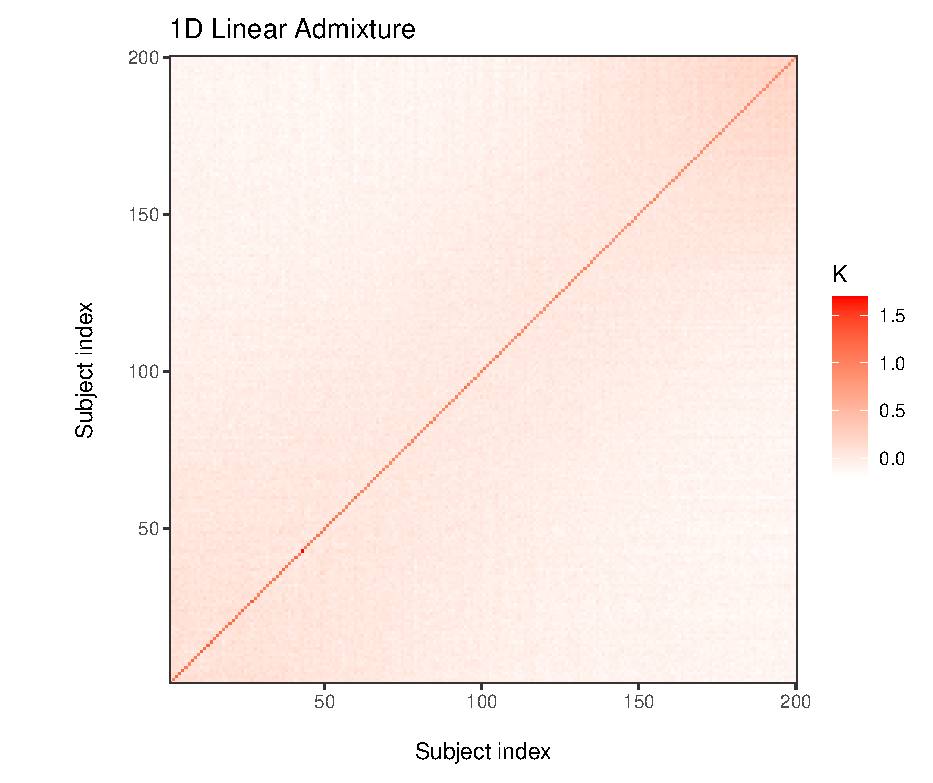
\includegraphics[scale = 1]{figures/admixed_kinship.eps}
    \caption{1D Linear Admixture with coarse subpopulation structure (4 subpopulations, 50 subjects per subpopulation), RRM.}
    \label{fig:admixed}
\end{figure}

% INDEPENDENT SUBPOPULATIONS, COARSE, KINSHIP
\begin{figure}[H]
    \centering
    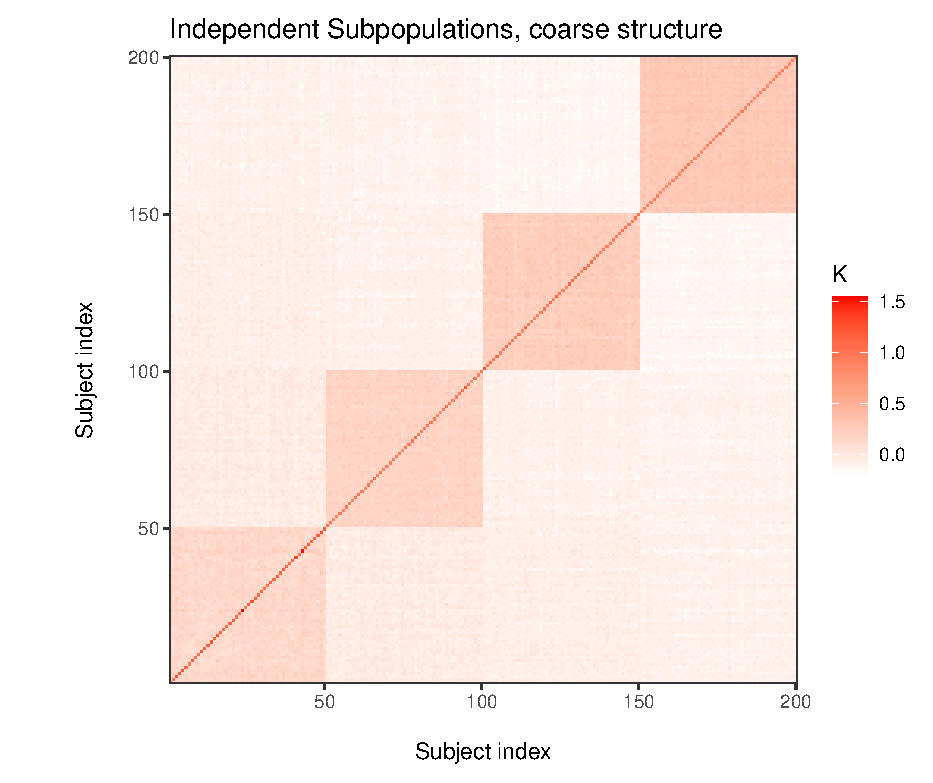
\includegraphics[scale = 1]{figures/indep_coarse_kinship.eps}
    \caption{Independent Subpopulations with coarse subpopulation structure (4 subpopulations, 50 subjects per subpopulation), RRM.}
    \label{fig:indep_coarse}
\end{figure}

% INDEPENDENT SUBPOPULATIONS, FINE, KINSHIP
\begin{figure}[H]
    \centering
    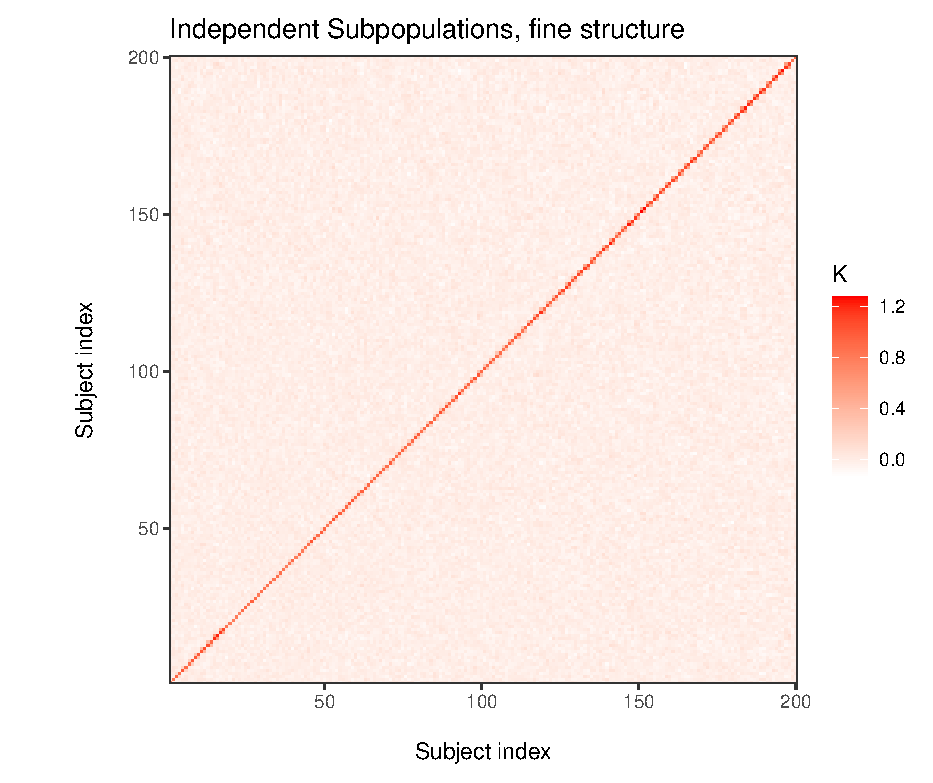
\includegraphics[scale = 1]{figures/indep_fine_kinship.eps}
    \caption{Independent Subpopulations with fine subpopulation structure (100 subpopulations, 2 subjects per subpopulation), RRM.}
    \label{fig:indep_fine}
\end{figure}

% EMPIRICAL KINSHIP
\begin{figure}[H]
    \centering
    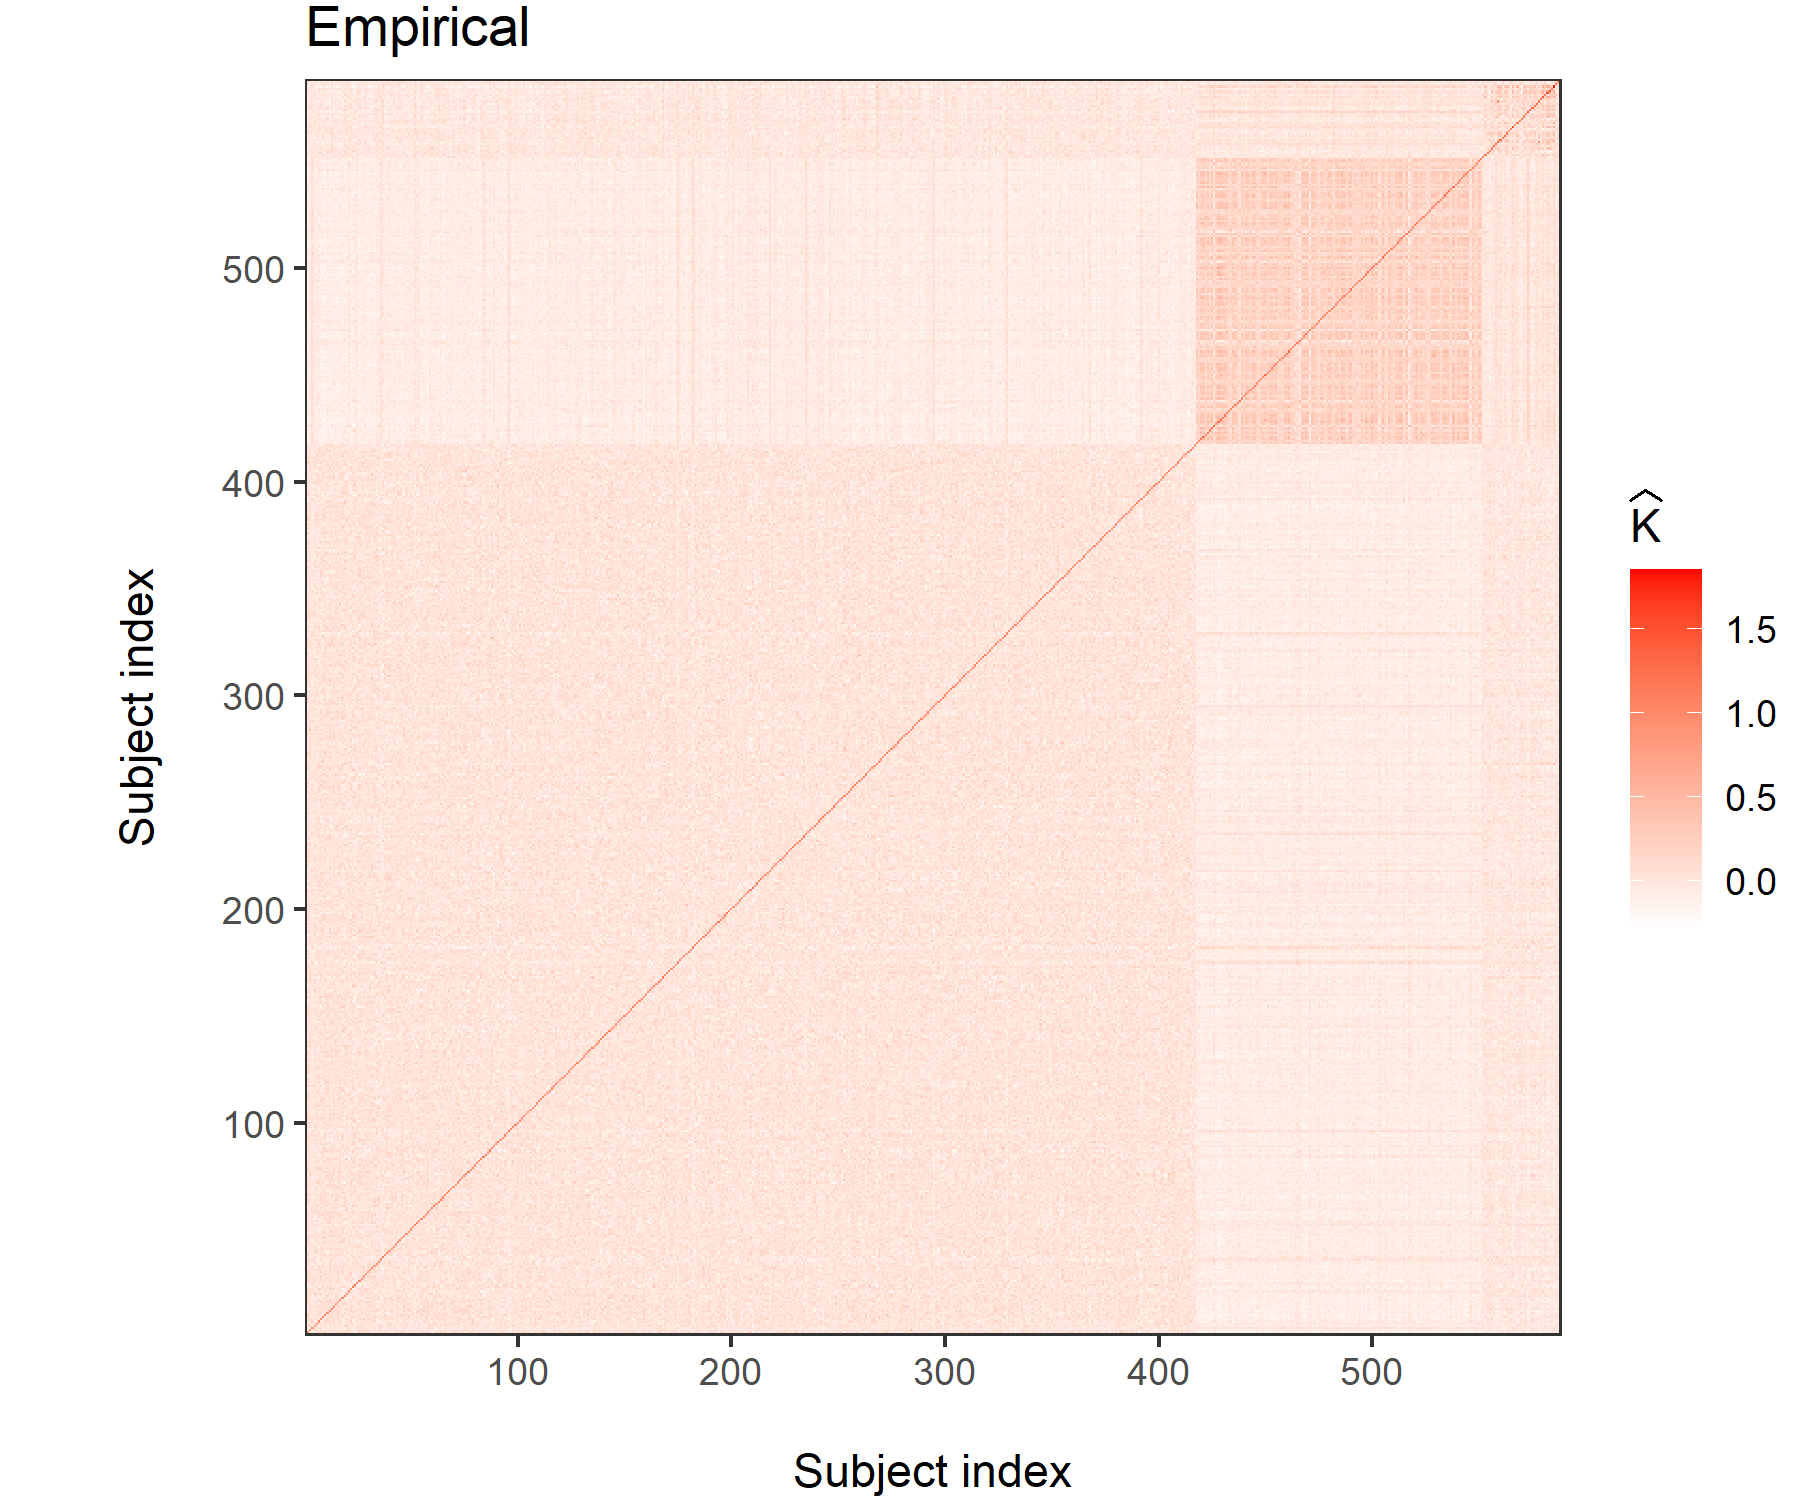
\includegraphics[scale = 1]{figures/empirical_kinship.eps}
    \caption{Empirical RRM.}
    \label{fig:empirical}
\end{figure}


\begin{sidewaysfigure}
    \centering
    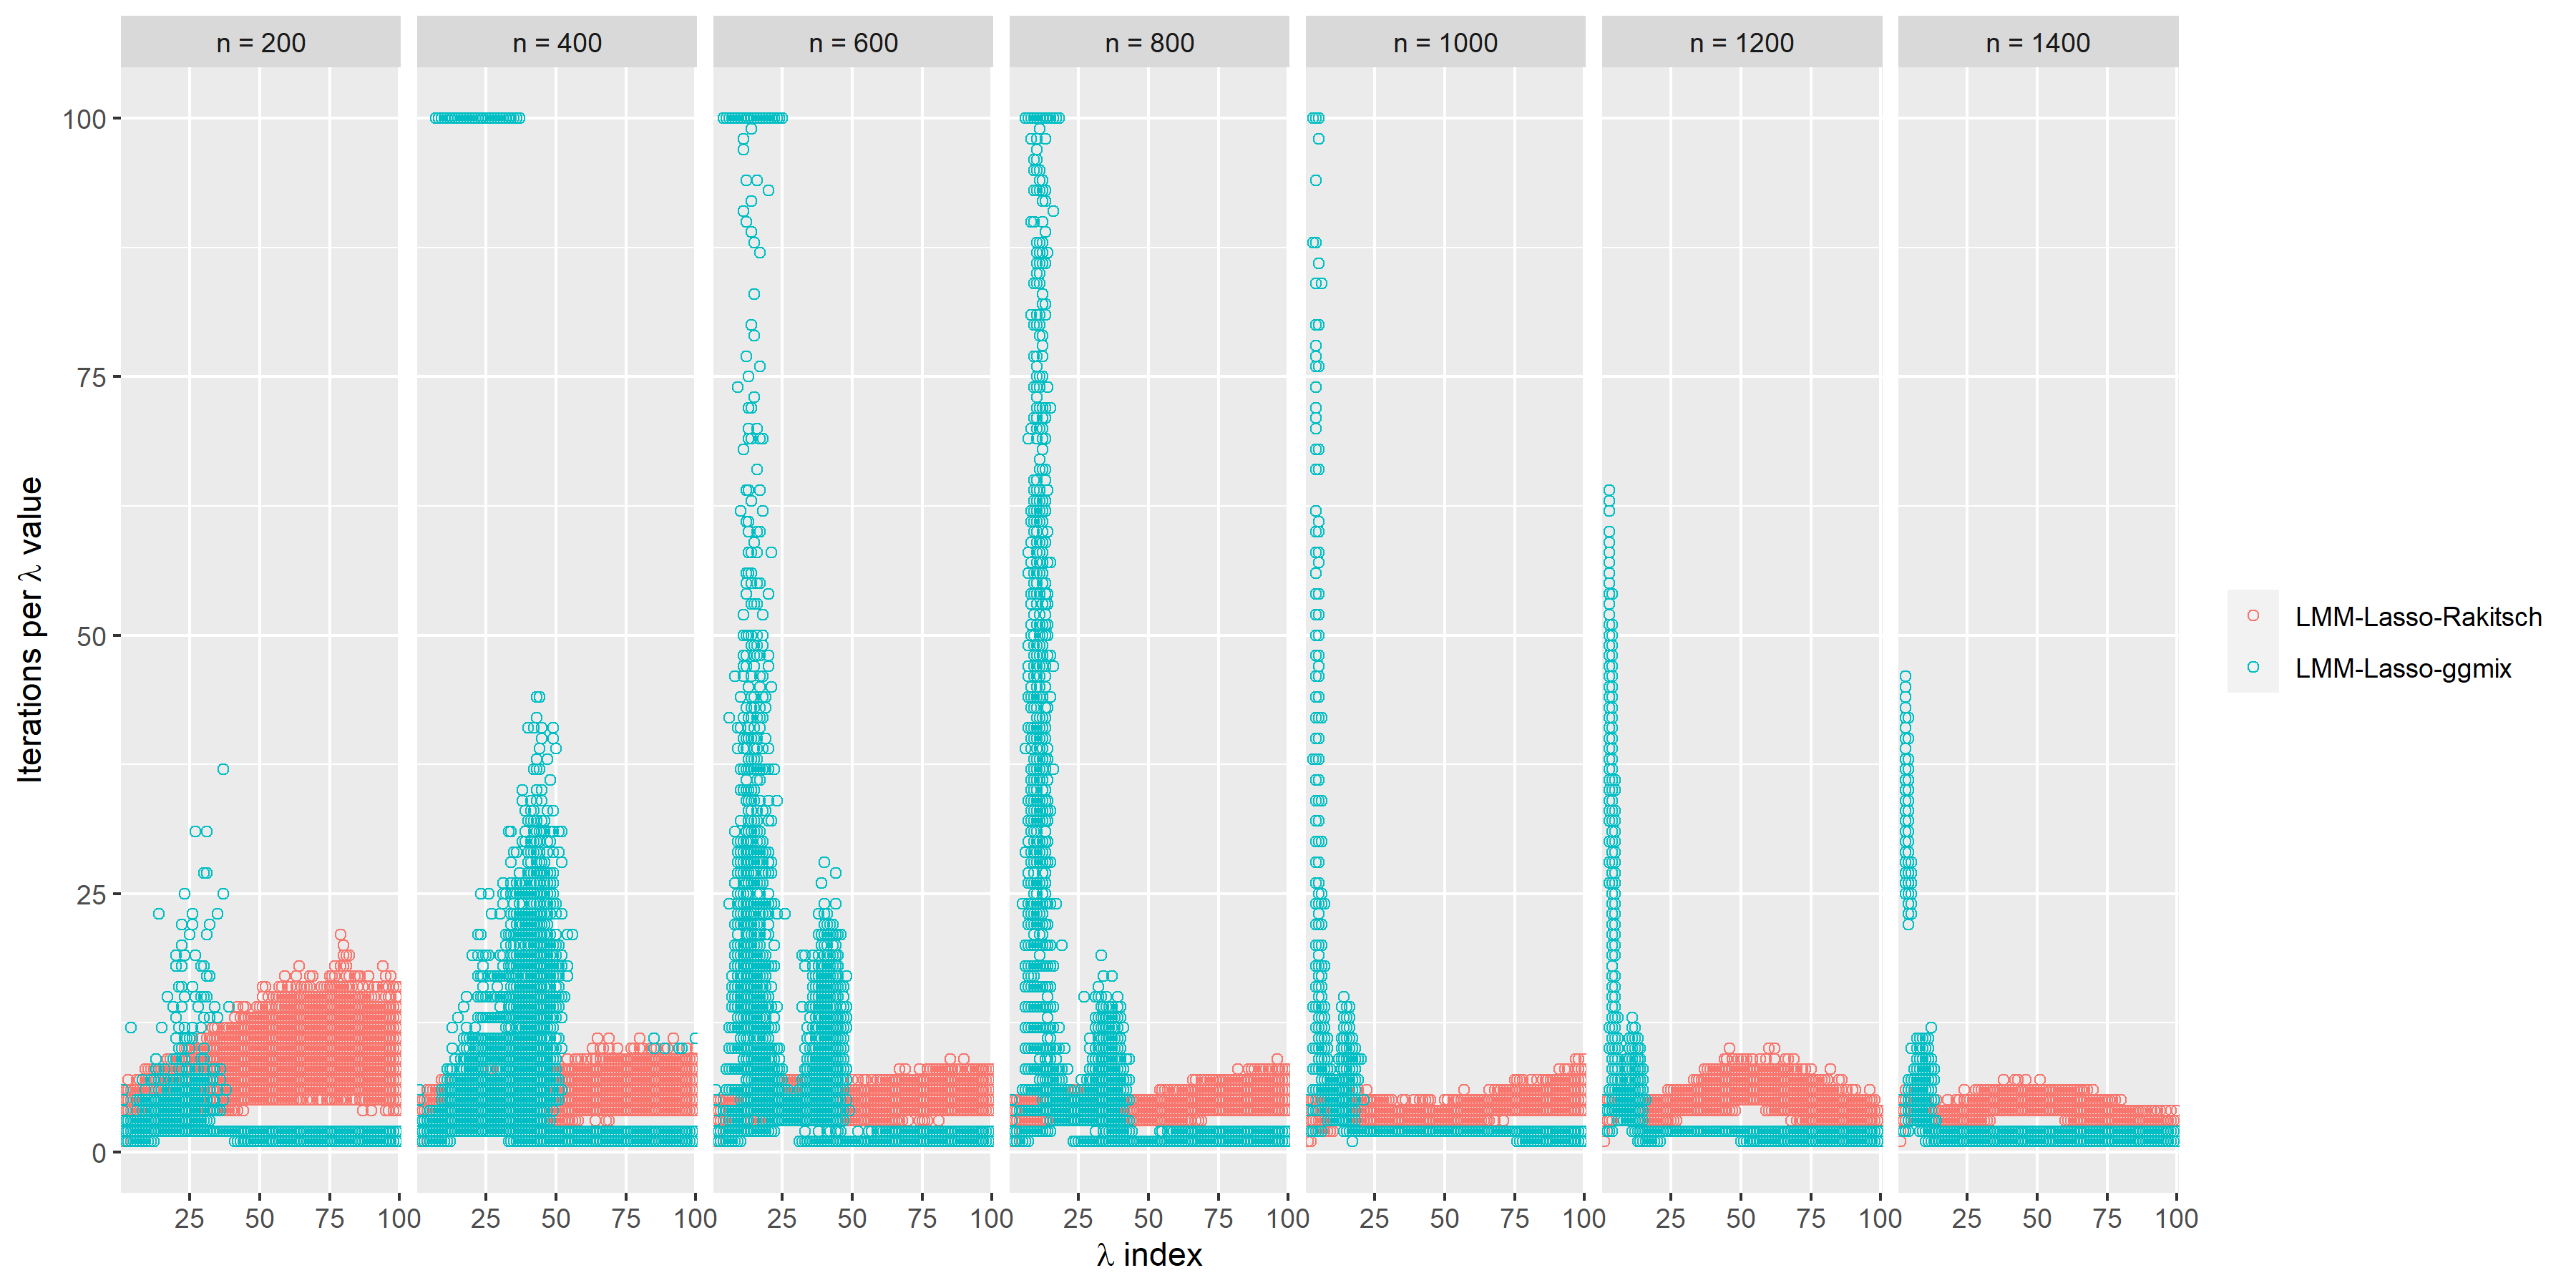
\includegraphics[width=\textwidth, height=\textheight, keepaspectratio]{figures/niter_perLambda_point.png}
    \caption{The number of iterations per $\lambda$ value for LMM-lasso-Rakitsch and LMM-lasso-ggmix across varying sample sizes with Independent Subpopulations data, coarse subpopulation structure, $\eta = 0.8$, and $\xi = 0.8$, and dichotomous-discordant environmental effect structure. Note that 100 is the maximum number of iterations for both implementations of LMM-lasso, so that numerous incidences of 100 iterations may indicate lack of model convergence.}
    \label{fig:niter}
\end{sidewaysfigure}


\end{document}
